\section{Atividade -- Bypass de Filtro de Upload}

\paragraph{}
Foi realizada a análise da funcionalidade de upload de arquivos da aplicação
\texttt{vulneravel.com} com o nível de segurança configurado para
\textit{Medium}.

\paragraph{}
Inicialmente foi criado um arquivo PHP contendo código para execução de
comandos no servidor, denominado \texttt{shell.php}. Ao tentar realizar o envio
normalmente, a aplicação bloqueou a operação informando que apenas arquivos dos
tipos JPEG e PNG eram permitidos.

\paragraph{}
Para contornar essa restrição foi utilizado o proxy de interceptação OWASP ZAP.
A requisição HTTP gerada pelo navegador foi interceptada e o cabeçalho
\texttt{Content-Type} do arquivo enviado foi alterado para \texttt{image/png},
mantendo o conteúdo original do arquivo PHP.

\paragraph{}
Após o encaminhamento da requisição modificada, a aplicação aceitou o envio do
arquivo e o armazenou no servidor, demonstrando que a validação do tipo de
arquivo era baseada apenas no valor informado pelo cliente.

\begin{figure}[H]
    \centering
    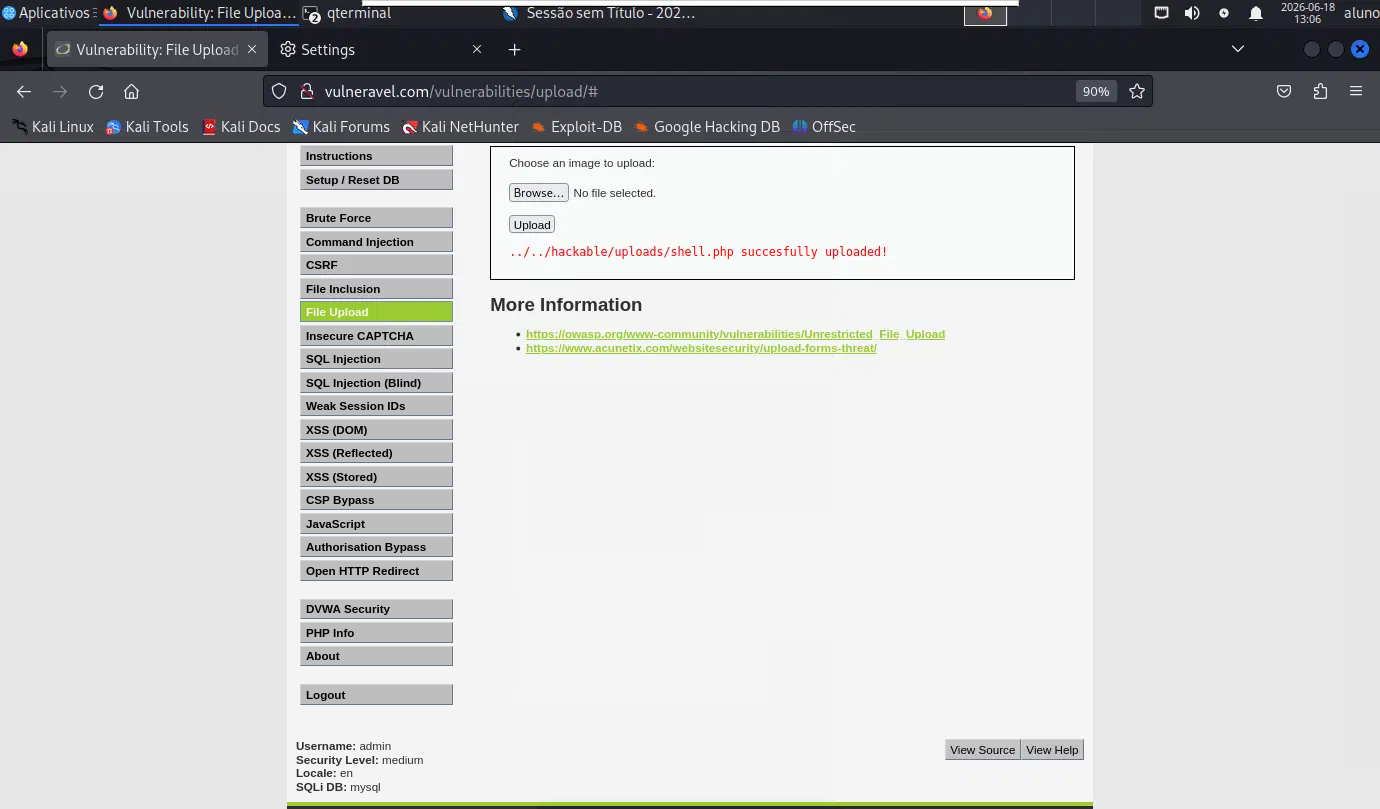
\includegraphics[width=0.95\textwidth]{./fig/upload-shell-medium.png}
    \caption{Aplicação configurada com nível de segurança Medium e envio
    bem-sucedido do arquivo \texttt{shell.php}.}
\end{figure}

\paragraph{}
A evidência demonstra que o mecanismo de validação implementado não realiza
verificações adequadas do conteúdo real do arquivo enviado, permitindo o upload
de código executável por meio da manipulação da requisição HTTP.
